%%%%%%%%%%%%%%%%%%%%%%%%%%%%%%%%%%%%%%%%%
% Lachaise Assignment
% LaTeX Template
% Version 1.0 (26/6/2018)
%
% This template originates from:
% http://www.LaTeXTemplates.com
%
% Authors:
% Marion Lachaise & François Févotte
% Vel (vel@LaTeXTemplates.com)
%
% License:
% CC BY-NC-SA 3.0 (http://creativecommons.org/licenses/by-nc-sa/3.0/)
% 
%%%%%%%%%%%%%%%%%%%%%%%%%%%%%%%%%%%%%%%%%

%----------------------------------------------------------------------------------------
%	PACKAGES AND OTHER DOCUMENT CONFIGURATIONS
%----------------------------------------------------------------------------------------

\documentclass{article}

%%%%%%%%%%%%%%%%%%%%%%%%%%%%%%%%%%%%%%%%%
% Lachaise Assignment
% Structure Specification File
% Version 1.0 (26/6/2018)
%
% This template originates from:
% http://www.LaTeXTemplates.com
%
% Authors:
% Marion Lachaise & François Févotte
% Vel (vel@LaTeXTemplates.com)
%
% License:
% CC BY-NC-SA 3.0 (http://creativecommons.org/licenses/by-nc-sa/3.0/)
% 
%%%%%%%%%%%%%%%%%%%%%%%%%%%%%%%%%%%%%%%%%

%----------------------------------------------------------------------------------------
%	PACKAGES AND OTHER DOCUMENT CONFIGURATIONS
%----------------------------------------------------------------------------------------

\usepackage{amsmath,amsfonts,amssymb} % Math packages

\usepackage{enumerate} % Custom item numbers for enumerations

\usepackage[ruled]{algorithm2e} % Algorithms

\usepackage[framemethod=tikz]{mdframed} % Allows defining custom boxed/framed environments

\usepackage{listings} % File listings, with syntax highlighting

\usepackage{booktabs}

\usepackage{graphicx}

\usepackage{caption}

\usepackage{subcaption}

\usepackage[T1]{fontenc}
\usepackage[utf8]{inputenc}
\usepackage{tikz}
\usetikzlibrary{shadows}

\usepackage[official]{eurosym}


\newcommand*\keystroke[1]{%
  \tikz[baseline=(key.base)]
    \node[%
      draw,
      fill=white,
      drop shadow={shadow xshift=0.25ex,shadow yshift=-0.25ex,fill=black,opacity=0.75},
      rectangle,
      rounded corners=2pt,
      inner sep=1pt,
      line width=0.5pt,
      font=\scriptsize\sffamily
    ](key) {#1\strut}
  ;
}


%----------------------------------------------------------------------------------------
%	DOCUMENT MARGINS
%----------------------------------------------------------------------------------------

\usepackage{geometry} % Required for adjusting page dimensions and margins
\setlength\parindent{0pt}
\geometry{
	paper=a4paper, % Paper size, change to letterpaper for US letter size
	top=2.5cm, % Top margin
	bottom=3cm, % Bottom margin
	left=2.5cm, % Left margin
	right=2.5cm, % Right margin
	headheight=14pt, % Header height
	footskip=1.5cm, % Space from the bottom margin to the baseline of the footer
	headsep=1.2cm, % Space from the top margin to the baseline of the header
	%showframe, % Uncomment to show how the type block is set on the page
}

%----------------------------------------------------------------------------------------
%	FONTS
%----------------------------------------------------------------------------------------

\usepackage[utf8]{inputenc} % Required for inputting international characters
\usepackage[T1]{fontenc} % Output font encoding for international characters

\usepackage{XCharter} % Use the XCharter fonts

%----------------------------------------------------------------------------------------
%	COMMAND LINE ENVIRONMENT
%----------------------------------------------------------------------------------------

% Usage:
% \begin{commandline}
%	\begin{verbatim}
%		$ ls
%		
%		Applications	Desktop	...
%	\end{verbatim}
% \end{commandline}

\mdfdefinestyle{commandline}{
	leftmargin=10pt,
	rightmargin=10pt,
	innerleftmargin=15pt,
	middlelinecolor=black!50!white,
	middlelinewidth=2pt,
	frametitlerule=false,
	backgroundcolor=black!5!white,
	frametitle={Command Line},
	frametitlefont={\normalfont\sffamily\color{white}\hspace{-1em}},
	frametitlebackgroundcolor=black!50!white,
	nobreak,
}

% Define a custom environment for command-line snapshots
\newenvironment{commandline}{
	\medskip
	\begin{mdframed}[style=commandline]
}{
	\end{mdframed}
	\medskip
}

%----------------------------------------------------------------------------------------
%	FILE CONTENTS ENVIRONMENT
%----------------------------------------------------------------------------------------

% Usage:
% \begin{file}[optional filename, defaults to "File"]
%	File contents, for example, with a listings environment
% \end{file}

\mdfdefinestyle{file}{
	innertopmargin=1.6\baselineskip,
	innerbottommargin=0.8\baselineskip,
	topline=false, bottomline=false,
	leftline=false, rightline=false,
	leftmargin=2cm,
	rightmargin=2cm,
	singleextra={%
		\draw[fill=black!10!white](P)++(0,-1.2em)rectangle(P-|O);
		\node[anchor=north west]
		at(P-|O){\ttfamily\mdfilename};
		%
		\def\l{3em}
		\draw(O-|P)++(-\l,0)--++(\l,\l)--(P)--(P-|O)--(O)--cycle;
		\draw(O-|P)++(-\l,0)--++(0,\l)--++(\l,0);
	},
	nobreak,
}

% Define a custom environment for file contents
\newenvironment{file}[1][File]{ % Set the default filename to "File"
	\medskip
	\newcommand{\mdfilename}{#1}
	\begin{mdframed}[style=file]
}{
	\end{mdframed}
	\medskip
}

%----------------------------------------------------------------------------------------
%	NUMBERED QUESTIONS ENVIRONMENT
%----------------------------------------------------------------------------------------

% Usage:
% \begin{question}[optional title]
%	Question contents
% \end{question}

\mdfdefinestyle{question}{
	innertopmargin=1.2\baselineskip,
	innerbottommargin=0.8\baselineskip,
	roundcorner=5pt,
	nobreak,
	singleextra={%
		\draw(P-|O)node[xshift=1em,anchor=west,fill=white,draw,rounded corners=5pt]{%
		Question \theQuestion\questionTitle};
	},
}

\newcounter{Question} % Stores the current question number that gets iterated with each new question

% Define a custom environment for numbered questions
\newenvironment{question}[1][\unskip]{
	\bigskip
	\stepcounter{Question}
	\newcommand{\questionTitle}{~#1}
	\begin{mdframed}[style=question]
}{
	\end{mdframed}
	\medskip
}

%----------------------------------------------------------------------------------------
%	WARNING TEXT ENVIRONMENT
%----------------------------------------------------------------------------------------

% Usage:
% \begin{warn}[optional title, defaults to "Warning:"]
%	Contents
% \end{warn}

\mdfdefinestyle{warning}{
	topline=false, bottomline=false,
	leftline=false, rightline=false,
	nobreak,
	singleextra={%
		\draw(P-|O)++(-0.5em,0)node(tmp1){};
		\draw(P-|O)++(0.5em,0)node(tmp2){};
		\fill[black,rotate around={45:(P-|O)}](tmp1)rectangle(tmp2);
		\node at(P-|O){\color{white}\scriptsize\bf !};
		\draw[very thick](P-|O)++(0,-1em)--(O);%--(O-|P);
	}
}

% Define a custom environment for warning text
\newenvironment{warn}[1][Warning:]{ % Set the default warning to "Warning:"
	\medskip
	\begin{mdframed}[style=warning]
		\noindent{\textbf{#1}}
}{
	\end{mdframed}
}

%----------------------------------------------------------------------------------------
%	INFORMATION ENVIRONMENT
%----------------------------------------------------------------------------------------

% Usage:
% \begin{info}[optional title, defaults to "Info:"]
% 	contents
% 	\end{info}

\mdfdefinestyle{info}{%
	topline=false, bottomline=false,
	leftline=false, rightline=false,
	nobreak,
	singleextra={%
		\fill[black](P-|O)circle[radius=0.4em];
		\node at(P-|O){\color{white}\scriptsize\bf i};
		\draw[very thick](P-|O)++(0,-0.8em)--(O);%--(O-|P);
	}
}

% Define a custom environment for information
\newenvironment{info}[1][Info:]{ % Set the default title to "Info:"
	\medskip
	\begin{mdframed}[style=info]
		\noindent{\textbf{#1}}
}{
	\end{mdframed}
}
 % Include the file specifying the document structure and custom commands

%----------------------------------------------------------------------------------------
%	ASSIGNMENT INFORMATION
%----------------------------------------------------------------------------------------

\title{Cost Comparison Tool Transportation Costs} % Title of the assignment

\author{W. de Zeeuw\\ \texttt{wessel.dezeeuw@tno.nl}} % Author name and email address

\date{TNO, Utrecht --- \today} % University, school and/or department name(s) and a date

%----------------------------------------------------------------------------------------

\begin{document}

\maketitle % Print the title

%----------------------------------------------------------------------------------------
%	INTRODUCTION
%----------------------------------------------------------------------------------------

\section*{Introduction} % Unnumbered section

	This tool is developed for TNO. The main goal for this tool is to make a
    comparison of costs made in different electricity transportation scenarios.
    One of this scenarios consists of the costs made when captured wind energy
    is electrolized to H2, compressed and transported through a pipeline. A
    second scenarios is the direct transportation to the Dutch electricity net
    using electricity cables and either AD/DC currents.

\bigskip
\textit{Section in progress} 

\section{Installation and starting the application}
\subsection{Installation}
In this section the installation process for the Cost Comparison Tool will be explained. After this section the reader will have a proper version of the tool available for personal usa. The user is provide with a \texttt{.zip}-file which includes all the necessary files. In this \texttt{.zip}-file the user find the folder \texttt{for\_redistribution}. To install the tool, the user enters this folder and double clicks on the \texttt{.exe} -file inside this folder. This opens the installation procedure. Procede with the installation by reading the information and by clicking the \texttt{'Next >'} button. In the next screen, the user may adapt the defaul installation folder and choose for the option to add a shortcut to the desktop (recommended). MATLAB Runtime is required for installation, but is included in the package. Finish installation by clicking the \texttt{'Install >'} button. 
\begin{info}
Admin rights are required for proper installation of the tool. The installation tool may ask for credentials. Also, do not close the screen. Closing the screen during installation will cause in a failed installation.
\end{info}

\begin{figure}[b!]
\centering
\begin{subfigure}{.5\textwidth}
  \centering
  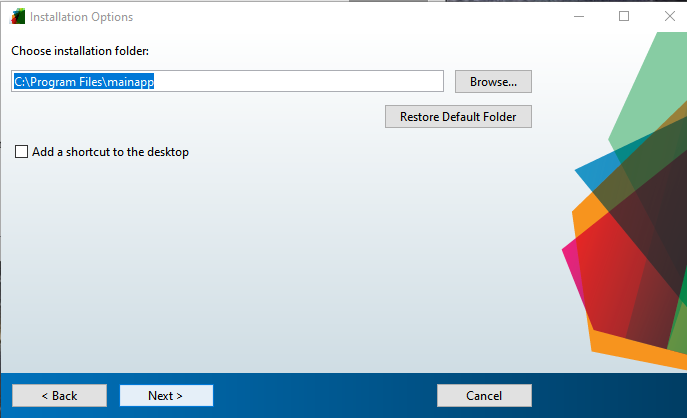
\includegraphics[width=.75\linewidth]{install1.png}
  \label{fig:sub1}
\end{subfigure}%
\begin{subfigure}{.5\textwidth}
  \centering
  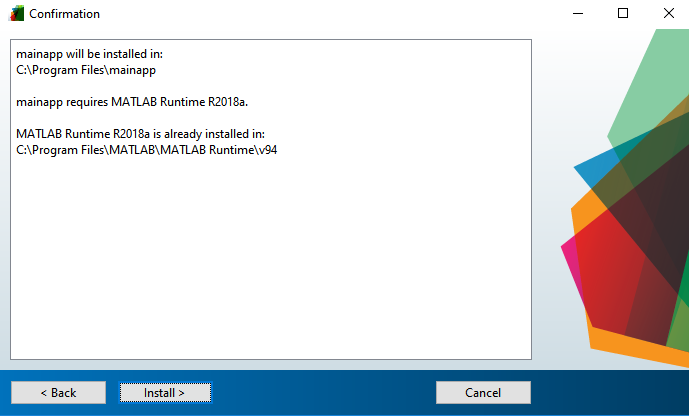
\includegraphics[width=.75\linewidth]{install2.png}
  \label{fig:sub2}
\end{subfigure}
\caption{The installation process}
\label{fig:install}
\end{figure}

A visualization of the procedure may be found in figure (\ref{fig:install})
\bigskip
\subsection{Deinstallation}
To remove the tool, press \keystroke{Windows} and type \texttt{Add or remove program}. This opens a window with different applications that may be removed. Find \texttt{TOET} in the list an click on this. Finally press the \keystroke{Uninstall}-button and follow the instructions on the screen. Only then the application is fully removed from your pc. A second way for deinstalling the package is by searching for the tool in the start menu. After the user has right-clicked, it will show an option to uninstall. Click this option and follow the instructions on the screen.
\begin{info}
Admin rights are required for proper deinstallation of the tool. The installation tool may ask for credentials.
\end{info}

\subsection{Starting the application}
Once the application has been installed it is ready to be used. You can open the application in many different ways, so we will limit ourselves to the most simple solutions.
\begin{enumerate}
\item Press the \keystroke{Windows} key on your keyboard  and type \texttt{ TOET} in the search area.  Clicking on the appearing result will open the application.
\item Double click on the shortcut created on your desktop.
\end{enumerate}

\begin{info}
If one of these options above doesn't work, the application can always be started, by going to folder specified during the installation phase.
\end{info}

\section{The application}

After opening, the user will be presented the homescreen of the application. The home screen tool consists of different buttons and panels, as visualized in figure (\ref{fig:open1}). One can find the following eight major components on the application

\begin{figure}[h]
  \centering
  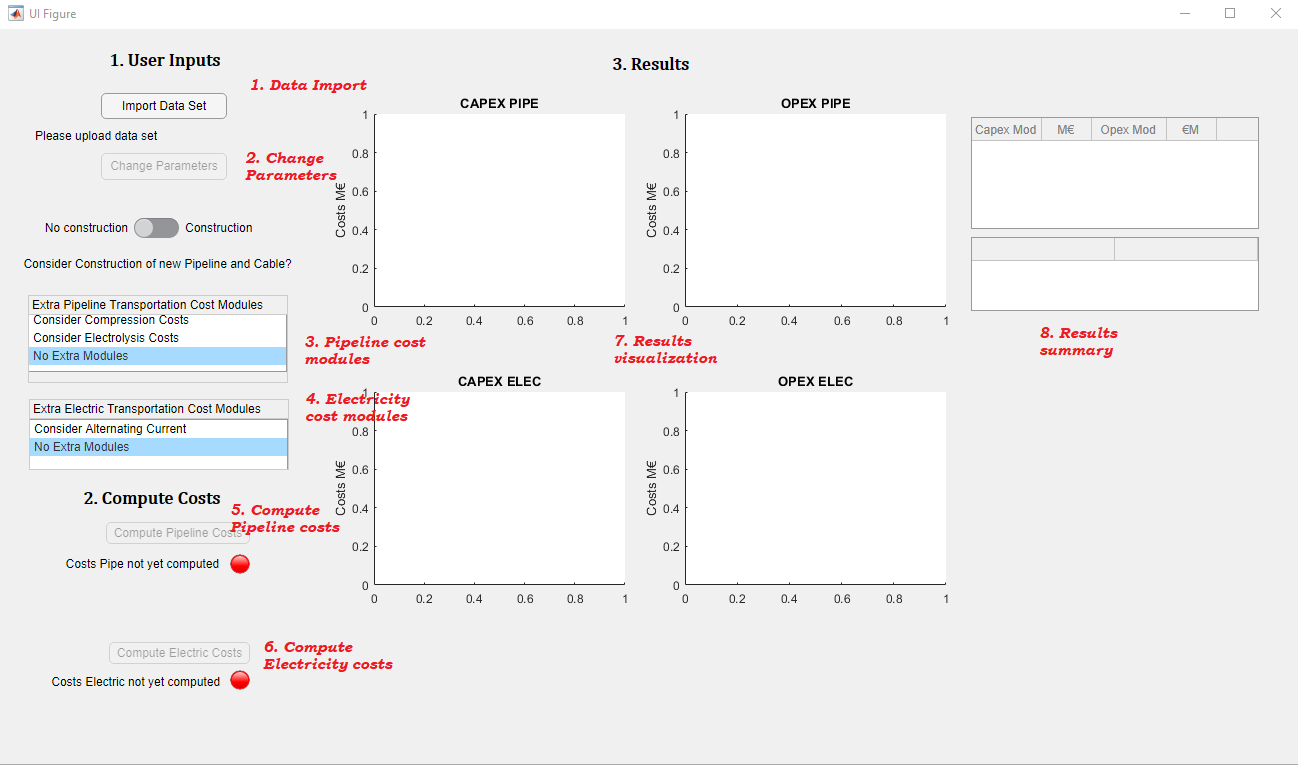
\includegraphics[width=.75\linewidth]{open1.png}
  \caption{The man screen of the application}
  \label{fig:open1}
\end{figure}


\begin{enumerate}
	\item Import dataset: use this button to import all the required variables, factors and constants.  
	\item Change parameters: use this button to change the primary variables of the system. 
	\item Pipeline Transportation Cost Modules: use this window to select all different options for the compution pipeline transportation costs.
	\item Electric Energy Transportation Cost Modules: use this window to select all different options for the computation of electricity transportation costs.
	\item Compute Pipeline Costs: use this button to calculate, or update, the costs for pipeline transportation.
	\item Compute Electric Costs: use this button to calculate, or update, the costs for electric transportation.
	\item Visualization of the calculated results.
	\item Summary of all the results
\end{enumerate}

By default, the user is unable to click on all buttons except for the \texttt{'Import Data Set'}. Also, the result panes are empty. Next to this, the applications will show if the computation raises any warnings that are interesting for the user. This is indicated by the light indicators and the spaced below the indicator lights. In the next sections, we will more thouroughly explain each of the requirements, functions and assumptions within each module. 

\subsection{Import dataset}
As mentioned before, this button will allows the user to import all required (default) values of the variables, factors and constants. The imported file must be of an \texttt{*.xlsx}-extention. The user is supplied with a default \texttt{*.xlsx} file that should be used. The lay-out of the input file is visualized in figure (\ref{fig:input1.png}).
\begin{warn}
	It must be noticed that none of the variables in the supplied dataset can be deleted. All inputs are used in the system, hence removing this data will lead to a system error. Next to this, the user is not allowed to change anything except for the values of the variables. This is prevented as the file is locked for changes, with exception of the value column.
\end{warn}
 
 After a successful upload of the datafile, the user will be notified of this by a \texttt{'Upload successful!'} statement. If this is the case, the buttons \texttt{'Compute Pipeline Costs'} and \texttt{'Compute Electric Costs'} become available. Else, the user is supplied with a \texttt{'Upload not successful!'} statement. In this case the user should supply the tool with a different dataset.
 
 \begin{warn}
 	The user must upload a dataset in order for the tool to work! If not, the user will not be able 
 \end{warn}

\begin{figure}[b!]
  \centering
  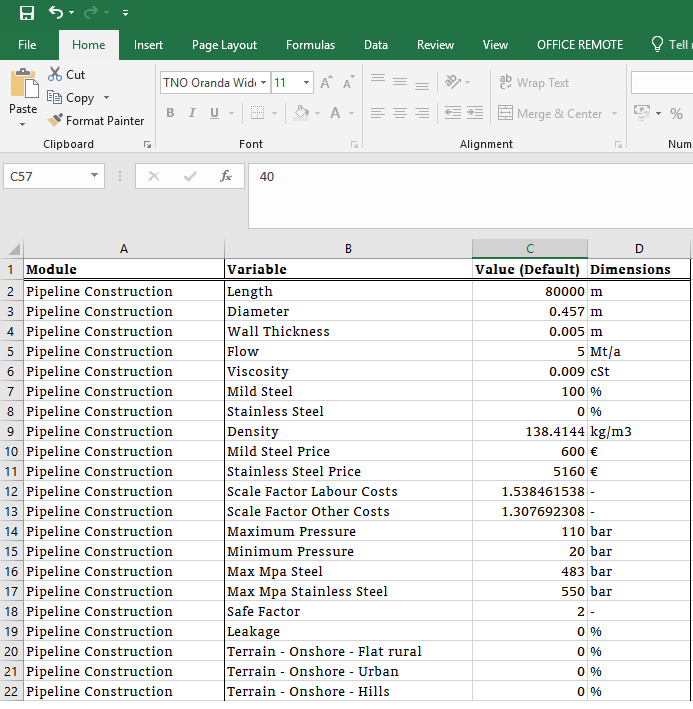
\includegraphics[width=.63\linewidth]{input1.png}
  \caption{The structure of the input file}
  \label{fig:input1}
\end{figure}

\subsection{Change Parameters}
By clicking on this button, the user is able to change any of the main variables of the program. The inputs that are changable for the user can be found in table [\ref{table:Inputs}].
\begin{table}[h]
\centering
\begin{tabular}{@{}lll@{}}
\toprule
Variable              & Default Value & Dimension \\ \midrule
Project Duration      & 20            & years     \\
Pipeline Length       & 80            & km        \\
Design Flow           & 5             & Mt/a      \\
Max. Pressure         & 110           & bar       \\
Min. Input Pressure   & 20            & bar       \\
Discount Rate         & 7             & \%        \\
Utilization Rate Flow & 70            & \%        \\
Mild Steel            & 100           & \%        \\
Stainless Steel       & 0             & \%        \\
Crossings             & 0             & -         \\
Terrain               & -             & -        
\end{tabular}
\caption{Changable Inputs}
\label{table:Inputs}
\end{table}

The application will open a different window in which the paramters can be updated. The window representation is visualized in figure (\ref{fig:param1}). Each component of the screen shows the current value of the parameter. Each parameter may be adaptable within a certain range. You can change the values for the project duration, pipeline and design flow rate by sliding the corresponding slider into the required value. Turning the knob to the required value has the same effect for the Discount- and Utilization ratew. To enable different configurations, press the switch. This enables the user to input different steel compositions. The user may, if desired, change the number of crossings or terrain composition.
\begin{info}
	It may be, that the \texttt{'Update'} button is unavailable. If this is the case, then there is a fault in the user defined changes. Please make sure that the Pipeline configuration and Terrain settings add up to $100\%$ in total for each categories.
\end{info}
 After the user is happy with the changes made, the user must confirm the changes by pressing the \texttt{'Update'} button. After a successful parameter adaption the user can see the message \texttt{'Parameters updated successfully!'}. Next to this, updating the parameters changes the colors of the indicator lights to orange, indication that the main variables have been changed and that the costs must be recomputed to represent the current 
\begin{warn}
	Closing the screen by clicking the $(\times)$ will not save the changes.
\end{warn}
\begin{info}
	Currently, the main variables for the electricity modules are not represented in the figure as there has been no work done on this. This screen can easily be extended to also cover these variables.
\end{info}

\begin{figure}[ht!]
  \centering
  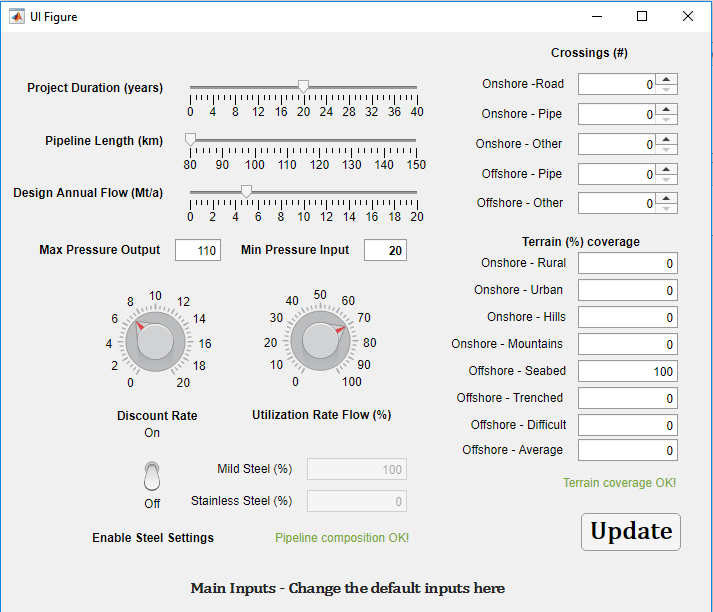
\includegraphics[width=.75\linewidth]{param1.png}
  \caption{The screen of the updating of the parameter}
  \label{fig:param1}
\end{figure}

\subsection{Pipeline Transportation Cost Modules}
This window allows the user to define which cost modules the user wants to consider. By default, the \texttt{'No extra modules'} is selected. This option may be changed by clicking on a different module. The modules may be supplemented with different modules by holding down the \keystroke{Ctrl}-button whilst clicking the required options. Any selected option can be disabled by clicking the required option once more, whilst pressing the \keystroke{Ctrl}-button. 
\begin{warn}
At least one module must be selected. Note that selection of \texttt{'No extra modules'} in combination with any different module means that this option gets neglected. Please note that the \texttt{'Electrolyse Costs'} module has not yet been implemented and hence will return a cost of $0$.
\end{warn}
Each module calculates the costs corresponding to the selected option.If more options are required, these can be added in this  We will discuss how the costs are calculated per module in. Here, the assumptions and sources can be found as well. Finally the costs are calculated by clicking on the \texttt{'Compute Pipeline Costs'}-button.

\subsection{Electric Energy Costs Transportation Cost Modules}
This module is equal to the Pipeline Transportation Cost Module. Hence, this window allows the user to define which cost modules the user wants to consider.  By default, the \texttt{'No extra modules'} is selected. This option may be changed by clicking on a different module. The modules may be supplemented with different modules by holding down the \keystroke{Ctrl}-button whilst clicking the required options. Any selected option can be disabled by clicking the required option once more, whilst pressing the \keystroke{Ctrl}-button. 
\begin{warn}
At least one module must be selected. Note that selection of \texttt{'No extra modules'} in combination with any different module means that this option gets neglected. Please note that the \texttt{'Electrolyse Costs'} module has not yet been implemented and hence will return a cost of $0$.
\end{warn}
Each module calculates the costs corresponding to the selected option.If more options are required, these can be added in this  We will discuss how the costs are calculated per module. Here, the assumptions and sources can be found as well.  Finally the costs are calculated by clicking on the \texttt{'Compute Electric Costs'}-button.

\section{Pipeline Transportation Cost Modules: Assumptions and Model}
In this section we will describe the formulae and assumptions made to compute the costs. As the modules may be selected independently

\subsection{Consider Costs for new Cable}
To compute all the costs corresponding to having a new cable, we must first determine the properties of our pipeline. All the variables and constants used can be found in table (\ref{table:Symbols}). The diameter of the pipeline is determined by a lookup table according to the formula
\begin{equation}
\dot{m} = \rho v_{avg} A \Rightarrow \dot{m} = \rho\pi D^2\sqrt{\frac{2D\Delta P_{allow}}{\nu\rho L}}
\end{equation}
Similarly, the wall stress is de
The maximum allowed pressure in MPa is denoted as
\begin{equation}
P_{max} = 
\begin{cases} 
483 \text{MPa } \quad \text{ if steel composition only includes mild steel}\\
550 \text{MPa } \quad \text{ if steel composition includes stainless steel}
\end{cases}
\end{equation}

The hoop stress is calculated according
\begin{equation}
\sigma_{\theta} = \frac{P_{in}D}{2w_t}  
\end{equation}
When $\sigma_{\theta} > \frac{P_{max}}{ SF}$, we conclude that the hoop stress is too high and may lead to dangerous situations.
\begin{info}
When the hoop stress is too high, this will lead to a warning message in the application. The user may decide wether or not to adjust the parameters to create a safe environment.
\end{info}

Similarly, we create a lookup table for the wall thickness of the diameter according to the formula
\begin{equation}
w_d = \frac{P_{max}D}{2\sigma_{theta}}
\end{equation}

Next to the hoop stess, we also require the pressure drop to be sufficiently small. To do this, we first calculate the velocity of the flow  in meters per second by
\begin{equation}
v_{f} = \frac{4f_R}{\pi D^2}, 
\end{equation}
where $f_R$ is the flow rate in cubic meters per second. With this velocity we may calculate the Reynolds number $\mathtt{Re}$. This number allows us to formulate the friction constant $\nu$. This gives 
\begin{equation}
\mathtt{Re} = \frac{v_fL}{\mu} \Rightarrow \nu = \begin{cases} \frac{64}{\mathtt{Re}} &\quad \text{if } \mathtt{Re} <2300\\
\frac{0.3164}{\mathtt{Re}^{\frac{1}{4}}}&\quad  \text{ else}
\end{cases} 
\end{equation}
Finally, one can calculate the pressure drop $\Delta P_{allow}$ in MPa by rewriting
\begin{equation}
\Delta P = L\nu \frac{\rho}{2}\frac{v_f^2}{D}
\end{equation}
\begin{info}
When the pressure drop is too high, this will lead to a warning message in the application. The user may decide wether or not to adjust the parameters to create a safe environment.
\end{info}
Next, we may cacluate the required material to construct the pipeline with aid of the following formula
\begin{equation}
M = 7850\pi Lw_d(D - w_d)
\end{equation}
This equation can be used to calculate the total material costs as
\begin{equation}
C_M = \frac{\left(S_mC_m +S_sC_s\right)M}{10^5}
\end{equation}
We use different scaling ratios to compute labour costs and other costs for pipelines. These costs are for the entire pipeline lenght. There are additional costs for pipes that are offshore. Finally, the crossing costs can be found by summing over all the different crossing types and there costs. Therefore the cost may be computed as such
\begin{equation}
\begin{cases}
C_L &= r_LM\\
C_O &= r_OM\\
C_C &= \sum_{i} (\text{crossing type})_i\cdot (\text{crossing cost type})_i\\
C_A &= (16 + 0.64L)p_{off}\\
\end{cases}
\end{equation}
Now, we still need to scale effectively towards the environment. Hence, the total CAPEX costs may be computed as
\begin{equation}
\text{CAPEX } =(s_{on}p_{on} + s_{off}p_{off})\cdot (C_M + C_L + C_O +C_A)
\end{equation}
 We do not scale the crossing costs as they already take the effect of the environment into account. The operating costs are calculated by
\begin{equation}
\text{OPEX}_f = \Delta t\cdot\text{CAPEX}\cdot OM_f, \quad \text{OPEX}_{var} = \Delta \dot{m} OM_{var}
\end{equation}

\begin{table}[h!]
\parbox{0.45\linewidth}{
\centering
\begin{tabular}[t]{@{}lll@{}}
\toprule
Variable              &  	Symbol  & Dimension \\ \midrule
Pipeline Diameter & $D$ &  m \\
Pipeline Length &$L$& m\\
Pipeline Thickness & $w_d$ & m \\
Project Duration &$\Delta t$& a\\
Maximum Pressure & $P_{max}$ & MPa \\
Minimum Pressure & $P_{min}$ &bar \\
Pressure Drop & $ \Delta P$& bar \\
Maximum Pressure Drop & $ \Delta P_{allow}$ &bar \\
Safety Factor & $ SF$ & - \\
Hoop Stress & $\sigma_{\theta}$ & MPa \\
Velocity of Flow & $v_f$ & m/s \\
Velocity average &$v_{avg}$& m/s\\
Transported Flow &$\dot{m} $& Mt/a\\
Area &$ A $& m2\\
Flow Rate & $f_r$ & m3/s \\
Friction Constant &$  \nu $ & - \\
Reynolds Number & $\mathtt{Re} $ & - \\
Material Required & $M$ & kg \\
Fraction of Stainless Steel &$ S_s $ &\%\\
\end{tabular}
}
\hfill
\parbox{0.45\linewidth}{
\centering
\begin{tabular}[t]{@{}lll@{}}
\toprule
              &  	Symbol  & Dimension \\ \midrule
Density & $\rho$ & kg/m3 \\
Fraction of Mild Steel &$ S_m $& \%\\
Cost of Stainless Steel &$ C_s $& \euro{} \\
Cost of Mild Steel &$ C_m$ & \euro{}\\
Total Material Costs &$C_M$ & M\euro{}\\
Total Crossing Costs &$C_C$ & M\euro{}\\
Total Labour Costs &$C_L$ & M\euro{}\\
Tota Other Costs &$C_O$ & M\euro{}\\
Total Additional Costs &$C_A$ & M\euro{}\\
Scaling Factor Labour Costs & $r_L$ & - \\
Scaling Factor Other Costs & $r_O$ & - \\
Fraction of Onshore pipe &$p_{on}$& \% \\
Fraction of Offshore pipe &$p_{off}$& \%\\
Scaling factor terrain onshore &$s_{on}$& - \\
Scaling factor terrain offshore &$s_{off}$& - \\
Fixed percentage for Fixed OPEX &$OM_f$& \%\\
Fixed percentage forVariable OPEX &$OM_{var}$& \%\\
CAPEX& - & M€\\
OPEX (fixed or variable)& - & M€\\
\end{tabular}
}
\caption{Symbols and their respective meaning}
\label{table:Symbols}
\end{table}
\subsection{Costs for Compression}
This specific module, calculates the costs required for the compression of H$_2$ so that it satisfies the minimal pressure requirements. This section can be enabled manually in the selection screen. The variables and constants are denoted in table (\ref{table:Symbols2})
\begin{info}
When the users presses the button to calculate the Pipeline costs, the program calculates wether or not compression is required. If it is not required, but the compression module is selected, the program will give a warning. When compression is required, but the compression module is not selected, the program will give a warning as well. 
\end{info}
The compressor constists of a number of trains, capable of compressing flow. The designed flow per each train is given by 
\begin{equation}
f_T = \frac{\dot{m}\gamma_{year}}{T}
\end{equation}
Next, we calculate if, and how much compression is required from
\begin{equation}
\beta = \max \left( \max (P_D, P_{min}) - (P_{max} - \Delta P)  , 0 \right).
\end{equation}
We say that compression is required by $\beta >0$ bar. 
The costs for the compressor is calculated from
\begin{equation}
\text{CAPEX } = I_0\cdot\left(\frac{\beta}{W_0}\right)^yT^{me}, \text{OPEX}_f =\Delta t OM_f\cdot \text{CAPEX}
\end{equation}
It remains to calculate the energy required from the compressor. We use a look-up table to find the required capacity for the compressor. The compression energy is calculated from
\begin{equation}
E_{comp} = R_{comp}\beta f_TT 
\end{equation}
Next we can calculate the yearly electricity costs from
\begin{equation}
E_{year} = 36000 E_{comp}R_{load}C_{elek}
\end{equation}
These electricty costs contibute to the variable OPEX costs, hence
\begin{equation}
\text{OPEX}_{var} = \Delta t E_{year}
\end{equation}

\begin{table}[h!]
\parbox{0.45\linewidth}{
\centering
\begin{tabular}[t]{@{}lll@{}}
\toprule
Variable              &  	Symbol  & Dimension \\ \midrule
Transported Flow &$\dot{m} $& Mt/a\\
Project Duration &$\Delta t$& a\\
Flow per train &$ f_T$& kg/s \\
Constant to convert years to second &$\gamma_{year}$& - \\
Number of trains &$T$& - \\
Minimum H$_2$ capture &H$_{2_{min}}$& kg/s\\
Maximum H$_2$ capture &H$_{2_{max}}$& kg/s\\
Maximum Pressure & $P_{max}$ &bar \\
Minimum Pressure & $P_{min}$ &bar \\
Pressure Drop & $ \Delta P$& bar \\
Default Pressure &$P_D$& bar\\
Initial Investment Costs &$I_0$& M€\\
\end{tabular}
}\hfill
\parbox{0.45\linewidth}{
\centering
\begin{tabular}[t]{@{}lll@{}}
\toprule
       &  	Symbol  & Dimension \\ \midrule
Base Scale of Compressor&$W_0$& MW\\
Scaling factor &$y$& -\\
Multiplication exponent &$ 0.9$& -\\
Amount of compression required &$\beta$& bar\\
Compression Energy&$E_{comp}$& MW \\
Compressor Load &$R_{load}$& hours\\
Yearly Electricity Required &$ E_{year}$& kJ/a\\
Elekctricity Costs &$C_{elek}$& euro/kJ\\ 
Fixed percentage for Fixed OPEX &$OM_f$& \%\\
Fixed percentage forVariable OPEX &$OM_{var}$& \%\\
CAPEX& - & M€\\
OPEX (fixed or variable)& - & M€\\
\end{tabular}
}
\caption{Symbols and their respective meaning for compression}
\label{table:Symbols2}
\end{table}
\subsection{Costs for Electrolysis}
The module for this has been investigated. However, the model is of very different order then the other results. 

\subsection{Sources}
The formulae in the sections above are derived from a couple of different sources. If any equations are unclear, references can be found in the found in the following files
\begin{enumerate}
\item ECCO Tool Pipeline Module, \textit{Obtained from D. Loeve}, \texttt{Filename: pipeline4.xlsx; ECCO Pipeline\_sens.xlsx}. 
\item Compresstion Module, \textit{From the Geocapacity project}, \texttt{Filename: Compression Module.xlsx}.
\item NSE 2 WP A, \textit{Obtained from J. Koornneef}, \texttt{Filename: NSE 2 WP A Model Draft Version.xlsx}.
\end{enumerate}

\section{Electric Transportation Cost Modules: Assumptions and Model}
\textit{To Do: Implementation of the modules}

\section{Results}
In this section we will explain the results visible to the user. The results are easily understandable. The graphs show the total composition and the fracture of each module to the total costs. This is done for the CAPEX and OPEX. A more detailed summary of all the costs is given in the table below the figures.
\begin{info}
The OPEX costs are for the entire project duration. If the user wants to know the yearly OPEX costs, please set the project duration to one year or divide by the project duration.
\end{info}
Finally we compute two more constants: The CAPES:OPEX ratio $r$ and the Cost Per Tonnes in Euro. These are calculated from
\begin{equation}
r = \frac{r_D\text{CAPEX}}{\left( 1 - \left( 1 + r_D\right)^{-\Delta t}\right)\text{ OPEX}},\quad  \text{EuroPerTonnes} =  \frac{r_D\text{CAPEX}}{\left( 1 - \left( 1 + r_D\right)^{-\Delta t} +\text{ OPEX} \right)\dot{m}},
\end{equation}
where $r_D$ is the discount rate. $\dot{m}$ is the desinged amount of flow and $\Delta t$ is the project duration. 
\begin{info}
Note that the OPEX costs in the fomula above are yearly, and not the total OPEX costs!
\end{info} 
A visualization of the results are found in figure (\ref{fig:results})

\begin{figure}[h!]
  \centering
  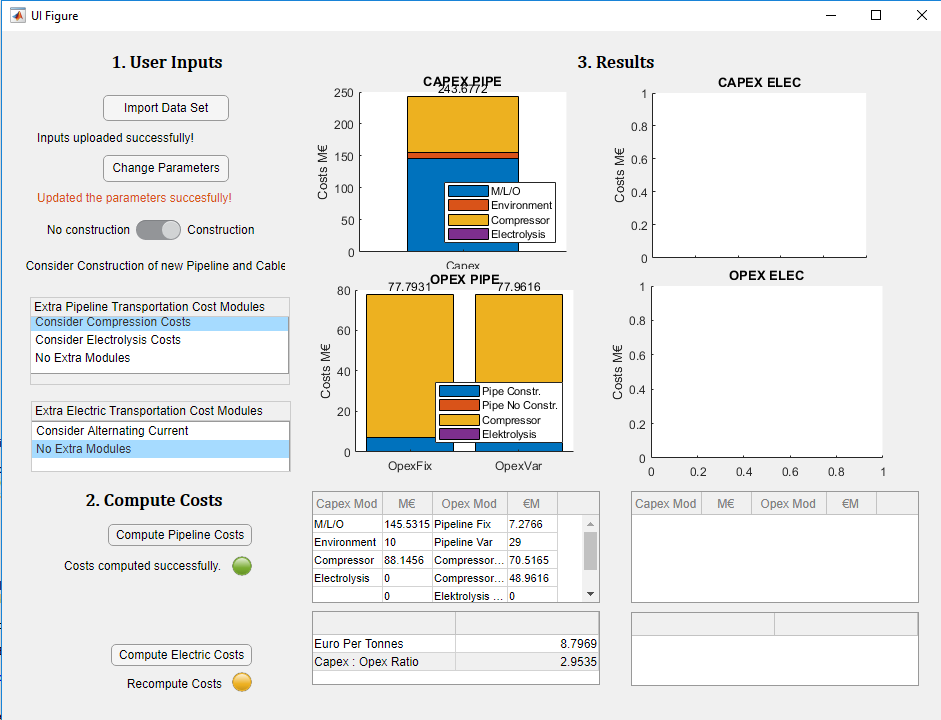
\includegraphics[width=.75\linewidth]{results.png}
  \caption{The results of the application}
  \label{fig:results}
\end{figure}

\end{document}